%%%%%%%%%%%%%%%%%%%%%%%%%%%%%%%%%%%%%%%%%%%%%%%%%%%%%%%%%%%
% --------------------------------------------------------
% Rho
% LaTeX Template
% Version 2.1.1 (01/09/2024)
%
% Authors: 
% Guillermo Jimenez (memo.notess1@gmail.com)
% Eduardo Gracidas (eduardo.gracidas29@gmail.com)
% 
% License:
% Creative Commons CC BY 4.0
% --------------------------------------------------------
%%%%%%%%%%%%%%%%%%%%%%%%%%%%%%%%%%%%%%%%%%%%%%%%%%%%%%%%%%%

\documentclass[10pt,a4paper,twoside]{rho-class/rho}
\usepackage[english]{babel}

% \usepackage{fontspec}  % Required for XeLaTeX and LuaLaTeX
% \setmainfont{Times New Roman} % Replace with any Unicode-supported font you want
\usepackage{xeCJK}  % For Chinese, Japanese, Korean characters (requires XeLaTeX)
% \setCJKmainfont{SimSun}  % Set to your preferred CJK font


%% Spanish babel recomendation
% \usepackage[spanish,es-nodecimaldot,es-noindentfirst]{babel}

\setbool{rho-abstract}{false} % Set false to hide the abstract
\setbool{corres-info}{false} % Set false to hide the corresponding author section

%----------------------------------------------------------
% TITLE
%----------------------------------------------------------

\journalname{Experiment on Computer Organization and Architecture}
\title{实验一:组合电路设计}

%----------------------------------------------------------
% AUTHORS AND AFFILIATIONS
%----------------------------------------------------------

\author {李雨轩}

%----------------------------------------------------------

\affil {西安交通大学}
\affil {计算机2205班}
\affil {2204112913}


%----------------------------------------------------------
% DATES
%----------------------------------------------------------

% \dates{This manuscript was compile on September 1, 2024}

%----------------------------------------------------------
% FOOTER INFORMATION
%----------------------------------------------------------

\leadauthor{计算机组成与结构专题实验}
\footinfo{COMP450905}
% \smalltitle{\LaTeX\ Template}
\institution{Xi'an Jiaotong University}
\theday{Oct 13, 2024} %\today

%----------------------------------------------------------
% ARTICLE INFORMATION
%----------------------------------------------------------

\corres{Provide the corresponding author information and publisher here.}
\email{example@organization.com.}
\doi{\url{https://www.doi.org/exampledoi/XXXXXXXXXX}}

\received{March 20, 2024}
\revised{April 16, 2024}
\accepted{April 20, 2024}
\published{May 21, 2024}

\license{Rho LaTeX Class \ccLogo\ This document is licensed under Creative Commons CC BY 4.0.}

%----------------------------------------------------------
% ABSTRACT
%----------------------------------------------------------

\begin{abstract}
    本实验的主要目的是通过使用 Vivado 软件和 Verilog  语言,设计和实现组合电路,包括基础门电路(多输入门电路、复用器)和基础功能模块(编码器、译码器)。在实验中,我们设计了多种组合电路,例如多输入门电路、二路复用器、八路复用器、基于三态缓冲器的四路复用器、8-3 编码器、8-3 优先编码器和 3-8 译码器。通过编写 Verilog 代码和 Testbench,对每个设计进行了仿真和验证,分析了仿真波形,验证了设计的正确性。实验加深了我们对组合逻辑电路的理解,培养了使用 Verilog 进行硬件描述和仿真的能力。
\end{abstract}

%----------------------------------------------------------

\keywords{Verilog, Vivado, FPGA, 数字系统设计}

%----------------------------------------------------------

\begin{document}
	
    \maketitle
    \thispagestyle{firststyle}
    % \tableofcontents
    % \linenumbers

%----------------------------------------------------------
\section{实验目的与实验内容}
    \rhostart{本}次实验主要内容为组合电路设计,包括基础门电路设计(多输入门电路、复用器)和基础功能模块设计(编码器、译码器)。实验内容如下:
    \begin {itemize}
        \item 用\verb|Vivado|实现基础门电路(多输入门电路、复用器等)的设计和测试;
        \item 用\verb|Vivado|实现基础功能模块(编码器、译码器等)的设计与测试。
    \end {itemize}

\section{实验要求}
    实验要求如下:
    \begin{itemize}
        \item 掌握\verb|Vivado|或Logisim开发工具的使用,掌握以上电路的设计和测试方法;
        \item 记录设计和调试过程(Verilog代码/电路图/表达式/真值表,\verb|Vivado|仿真结果,Logisim验证结果等);
        \item 分析\verb|Vivado|仿真波形/Logism验证结果,注重输入输出之间的对应关系。
    \end{itemize}

\section{实验过程及分析-1:基础门电路设计}
    基础门电路部分要求设计和测试一个给定表达式的多输入门电路和复用器,复用器将会包括一个简单的2路复用器、一个8路复用器,以及使用三态缓存器实现一个4路复用器。
    
    我在 \verb|Vivado| 中使用 Verilog 语言分别完成了多输入门电路(表达式已给定)、二路复用器、多路复用器(8路)以及使用三态缓存器实现的四路复用器的设计。通过仿真测试,验证了电路的逻辑正确性和时序关系。复用器设计体现了组合逻辑电路的选择功能,测试时各输入信号的变化可以实时反映在输出信号中。

    \subsection{多输入门电路}

        根据实验指导的要求,设计一个多输入门电路,逻辑表达式为:
        \[
        x = \overline{(a \cdot \overline{b} \cdot c \cdot (d + e))}
        \]
        
        \paragraph{Verilog 代码} 
            在\verb|Vivado|平台设计如下的Verilog代码(Code-\ref{lst:multi_input_gate}):
                \lstinputlisting[caption=多输入门电路设计代码., label={lst:multi_input_gate}, language=Verilog]{rtl/multi_input_gate.v}
        
        \paragraph{仿真testbench代码}
            为了验证电路设计的正确性,我编写了用于Behavioral Simulation的testbench。(Code-\ref{lst:tb_multi_input_gate}):
                \lstinputlisting[caption=多输入门电路testbench代码., label={lst:tb_multi_input_gate}, language=Verilog]{rtl/tb_multi_input_gate.v}
            在创建的TestBench文件中,我编写测试激励代码,代码每隔10ns更改一次输入,遍历每一个可能的输出(构造了 $2^5$ 个不同的五元组),以确保覆盖每一种输入。

        \paragraph{Behavioral Simulation输出波形}
            在 \verb|Vivado| 的 "Flow Navigator" 窗口中,找到 Simulation 部分,选择 Run Simulation。选择 Run Behavioral Simulation(行为仿真)。\verb|Vivado| 编译设计源代码和 Testbench,生成仿真文件,波形如            图 \ref{fig:tb_multi_input_gate} 所示。\footnote{出于排版美观的考量,多输入门电路的仿真波形(图 \ref{fig:tb_multi_input_gate})放在文章的最后}
        


        
    \subsection{二路复用器}
        根据实验指导的要求,设计一个二路复用器。二路复用器的逻辑表达式为:
        \[
        y = s \cdot d_1 + \overline{s} \cdot d_0
        \]
        其中,$d_0$ 和 $d_1$ 为两个数据输入,$s$ 为选择信号,$y$ 为输出。
        
        \paragraph{真值表}
        
            \[
            \begin{array}{|c|c|c!{\vrule width 1.4pt}c|}
            \hline
            S & D1 & D0 & Y \\
            \hline
            0 & 0 & 0 & 0 \\
            0 & 0 & 1 & 1 \\
            0 & 1 & 0 & 0 \\
            0 & 1 & 1 & 1 \\
            1 & 0 & 0 & 0 \\
            1 & 0 & 1 & 0 \\
            1 & 1 & 0 & 1 \\
            1 & 1 & 1 & 1 \\
            \hline
            \end{array}
            \]

        
        \paragraph{Verilog 代码}
        
            在 \verb|Vivado| 平台设计如下的 Verilog 代码(Code-\ref{lst:two_way_mux}):
                \lstinputlisting[caption=二路复用器设计代码., label={lst:two_way_mux}, language=Verilog]{rtl/two_way_mux.v}

        
        \paragraph{仿真 Testbench 代码}
        
            为了验证电路设计的正确性,我编写了用于 Behavioral Simulation 的 Testbench。(Code-\ref{lst:tb_two_way_mux}):
                \lstinputlisting[caption=二路复用器testbench代码., label={lst:tb_two_way_mux}, language=Verilog]{rtl/tb_two_way_mux.v}
        
        在创建的 Testbench 文件中,我编写了测试激励代码,代码每隔 10ns 更改一次输入,遍历每一种可能的输入组合(共 $2^3$ 个不同的三元组),以确保覆盖每一种输入情况。
        
        \paragraph{Behavioral Simulation 输出波形}
        
        在 \verb|Vivado| 的 "Flow Navigator" 窗口中,找到 Simulation 部分,选择 Run Simulation,选择 Run Behavioral Simulation(行为仿真)。\verb|Vivado| 编译设计源代码和 Testbench,生成仿真文件,波形如图 \ref{fig:tb_two_way_mux} 所示。\footnote{出于排版美观的考量,二路复用器的仿真波形(图 \ref{fig:tb_two_way_mux})放在文章的最后}
        



    \subsection{八路复用器}
        根据实验指导的要求,设计一个八路复用器。八路复用器的逻辑功能是根据选择信号选择一个输入信号作为输出。其逻辑表达式为:
        \[
        y = d_0 \cdot \overline{s_2} \cdot \overline{s_1} \cdot \overline{s_0} + d_1 \cdot \overline{s_2} \cdot \overline{s_1} \cdot s_0 + \dots + d_7 \cdot s_2 \cdot s_1 \cdot s_0
        \]
        
        
        \paragraph{Verilog 代码}
        
        在 \verb|Vivado| 平台设计如下的 Verilog 代码(Code-\ref{lst:eight_way_mux}):
                \lstinputlisting[caption=八路复用器设计代码., label={lst:eight_way_mux}, language=Verilog]{rtl/eight_way_mux.v}

        
        \paragraph{仿真 Testbench 代码}
        
            为了验证电路设计的正确性,我编写了用于 Behavioral Simulation 的 Testbench。(Code-\ref{lst:tb_eight_way_mux}):
                \lstinputlisting[caption=八路复用器testbench代码., label={lst:tb_eight_way_mux}, language=Verilog]{rtl/tb_eight_way_mux.v}
        
        
            在创建的 Testbench 文件中,我编写了测试激励代码,每隔 10ns 更改一次输入信号和选择信号,遍历所有可能的输入组合(共 $2^8 \cdot 2^3$ 种组合)。为了简化测试,这里选择了一些典型的输入组合,以确保覆盖每一种选择信号情况下的输出。
        
        \paragraph{Behavioral Simulation 输出波形}
        
            在 \verb|Vivado| 的 "Flow Navigator" 窗口中,找到 Simulation 部分,选择 Run Simulation,选择 Run Behavioral Simulation(行为仿真)。\verb|Vivado| 编译设计源代码和 Testbench,生成仿真文件,波形如图 \ref{fig:tb_eight_way_mux} 所示。\footnote{出于排版美观的考量,八路复用器的仿真波形(图 \ref{fig:tb_eight_way_mux})放在文章的最后}
        

    
    \subsection{基于三态缓存器的四路复用器}
        
        根据实验指导的要求,设计一个基于三态缓存器的4路复用器。该复用器有4个数据输入 $d_0$、$d_1$、$d_2$、$d_3$,2个选择输入 $s_1$、$s_0$,以及一个输出 $y$。利用三态缓存器实现,每次只有一个数据输入被选通到输出。
        
        三态缓存器的真值表如下:

            \[
            \begin{array}{|c|c!{\vrule width 1.4pt}c|}
            \hline
            E & A & Y \\
            \hline
            0 & 0 & Z \\
            0 & 1 & Z \\
            1 & 0 & 0 \\
            1 & 1 & 1 \\
            \hline
            \end{array}
            \]

        \paragraph{Verilog 代码}
        
        在 \verb|Vivado| 平台设计如下的 Verilog 代码(Code-\ref{lst:four_way_mux_tristate}):
                \lstinputlisting[caption=基于三态缓存器的四路复用器设计代码., label={lst:four_way_mux_tristate}, language=Verilog]{rtl/four_way_mux_tristate.v}

        
        \paragraph{仿真 Testbench 代码}
        
            为了验证电路设计的正确性,我编写了用于 Behavioral Simulation 的 Testbench。(Code-\ref{lst:tb_four_way_mux_tristate}):
                \lstinputlisting[caption=基于三态缓冲器的4路复用器testbench代码., label={lst:tb_four_way_mux_tristate}, language=Verilog]{rtl/tb_four_way_mux_tristate.v}


                
            在创建的 Testbench 文件中,我编写了测试激励代码,代码每隔 10ns 更改一次输入,遍历每一种可能的选择输入组合(共 $2^4 \cdot 2^2$ 个不同的二元组),并对每个通道进行测试,以确保覆盖每一种输入情况。
        
        \paragraph{Behavioral Simulation 输出波形}
        
            在 \verb|Vivado| 的 "Flow Navigator" 窗口中,找到 Simulation 部分,选择 Run Simulation,选择 Run Behavioral Simulation(行为仿真)。\verb|Vivado| 编译设计源代码和 Testbench,生成仿真文件,波形如图 \ref{fig:tb_four_way_mux_tristate} 所示。\footnote{出于排版美观的考量,基于三态缓存器的四路复用器的仿真波形(图 \ref{fig:tb_four_way_mux_tristate})放在文章的最后}
        




\section{实验过程及分析-2:基础功能模块设计}
    基础功能模块的设计分为两个部分,分别是编码器和译码器。对于编码器,将首先使用三种方式:行为描述方式、结构化描述和数据流描述分别实现一个简单的8-3编码器(非优先级编码器);然后再实现一个优先8-3编码器。对于译码器,将实现一个3-8译码器。
    
    \subsection{8-3编码器}
        
            根据实验指导的要求,设计一个8-3编码器,其功能是将8位输入信号编码为3位输出信号。当输入信号中有且仅有一位为高电平时,输出对应该高电平输入的位置编码。

        \paragraph{真值表}
        
            \[
            \begin{array}{|c|c|c|c|c|c|c|c!{\vrule width 1.4pt}c|c|c|}
            \hline
            D7 & D6 & D5 & D4 & D3 & D2 & D1 & D0 & Y2 & Y1 & Y0 \\
            \hline
            0 & 0 & 0 & 0 & 0 & 0 & 0 & 1 & 0 & 0 & 0 \\
            0 & 0 & 0 & 0 & 0 & 0 & 1 & 0 & 0 & 0 & 1 \\
            0 & 0 & 0 & 0 & 0 & 1 & 0 & 0 & 0 & 1 & 0 \\
            0 & 0 & 0 & 0 & 1 & 0 & 0 & 0 & 0 & 1 & 1 \\
            0 & 0 & 0 & 1 & 0 & 0 & 0 & 0 & 1 & 0 & 0 \\
            0 & 0 & 1 & 0 & 0 & 0 & 0 & 0 & 1 & 0 & 1 \\
            0 & 1 & 0 & 0 & 0 & 0 & 0 & 0 & 1 & 1 & 0 \\
            1 & 0 & 0 & 0 & 0 & 0 & 0 & 0 & 1 & 1 & 1 \\
            \hline
            \end{array}
            \]
        
        \paragraph{Verilog 代码} 
            在 \verb|Vivado| 平台设计如下的 Verilog 代码(Code-\ref{lst:encoder_8to3}):
                \lstinputlisting[caption=8-3编码器设计代码., label={lst:encoder_8to3}, language=Verilog]{rtl/encoder_8to3.v}

        
        \paragraph{仿真 Testbench 代码}
            为了验证电路设计的正确性,我编写了用于 Behavioral Simulation 的 Testbench。(Code-\ref{lst:tb_encoder_8to3}):
                \lstinputlisting[caption=8-3编码器testbench代码., label={lst:tb_encoder_8to3}, language=Verilog]{rtl/tb_encoder_8to3.v}
                
            在创建的 TestBench 文件中,我编写了测试激励代码,代码每隔 10ns 更改一次输入,遍历所有合法的输入(只有一位为1),以确保覆盖每一种输入情况。然后我又将代码\ref{lst:tb_encoder_8to3}的第14行中跳过非法输入的部分略去后,使用行为级描述设计的电路(见\ref{lst:tb_encoder_8to3}的第15行)再次进行测试,这时,对于非法输入,也能输出设定的值。
        
        \paragraph{Behavioral Simulation 输出波形}
            在 \verb|Vivado| 的 "Flow Navigator" 窗口中,找到 Simulation 部分,选择 Run Simulation。选择 Run Behavioral Simulation(行为仿真)。\verb|Vivado| 编译设计源代码和 Testbench,生成仿真文件,只有合法输入的波形如图 \ref{fig:tb_encoder_8to3} 所示,包含非法输入的波形如图 \ref{fig:tb_encoder_8to3_ill} 所示。\footnote{出于排版美观的考量,8-3编码器的仿真波形(图 \ref{fig:tb_encoder_8to3})放在文章的最后}
        

        
    \subsection{8-3优先编码器}

            根据实验指导的要求,设计一个8-3优先编码器。优先编码器用于将8位输入信号中最高有效位的位置编码为3位二进制数。当多个输入为高电平时,输出对应最高优先级的输入信号。
        
        \paragraph{真值表}
        
        \[
        \begin{array}{|c|c|c|c|c|c|c|c!{\vrule width 1.4pt}c|c|c|c|}
        \hline
        D7 & D6 & D5 & D4 & D3 & D2 & D1 & D0 & Y2 & Y1 & Y0 & V \\
        \hline
        0 & 0 & 0 & 0 & 0 & 0 & 0 & 0 & X & X & X & 0 \\
        0 & 0 & 0 & 0 & 0 & 0 & 0 & 1 & 0 & 0 & 0 & 1 \\
        0 & 0 & 0 & 0 & 0 & 0 & 1 & X & 0 & 0 & 1 & 1 \\
        0 & 0 & 0 & 0 & 0 & 1 & X & X & 0 & 1 & 0 & 1 \\
        0 & 0 & 0 & 0 & 1 & X & X & X & 0 & 1 & 1 & 1 \\
        0 & 0 & 0 & 1 & X & X & X & X & 1 & 0 & 0 & 1 \\
        0 & 0 & 1 & X & X & X & X & X & 1 & 0 & 1 & 1 \\
        0 & 1 & X & X & X & X & X & X & 1 & 1 & 0 & 1 \\
        1 & X & X & X & X & X & X & X & 1 & 1 & 1 & 1 \\
        \hline
        \end{array}
        \]
        
        其中,$D7$ 为最高优先级,$D0$ 为最低优先级;$Y2$、$Y1$、$Y0$ 为输出编码;$V$ 为有效位,当输入全为0时,$V=0$,输出无效。
        
        \paragraph{逻辑表达式}
        
        根据真值表,可以推导出输出的逻辑表达式:
            \begin{align*}
            Y2 &= D4 + D5 + D6 + D7 \\
            Y1 &= D2 + D3 + D6 + D7 \\
            Y0 &= D1 + D3 + D5 + D7 \\
            V &= D0 + D1 + D2 + D3 + D4 + D5 + D6 + D7
            \end{align*}
        
        
        \paragraph{Verilog 代码}
        
        在 \verb|Vivado| 平台设计如下的 Verilog 代码(Code-\ref{lst:priority_encoder_8to3}):
                \lstinputlisting[caption=8-3优先编码器设计代码., label={lst:priority_encoder_8to3}, language=Verilog]{rtl/priority_encoder_8to3.v}

        
        \paragraph{仿真 Testbench 代码}
        
            为了验证电路设计的正确性,我编写了用于 Behavioral Simulation 的 Testbench。(Code-\ref{lst:tb_priority_encoder_8to3}):
                \lstinputlisting[caption=8-3优先编码器testbench代码., label={lst:tb_priority_encoder_8to3}, language=Verilog]{rtl/tb_priority_encoder_8to3.v}

        
            在创建的 Testbench 文件中,我编写了测试激励代码,每隔 10ns 更改一次输入,遍历不同的输入组合,以确保覆盖每一种优先级输入。
        
        \paragraph{Behavioral Simulation 输出波形}
        
            在 \verb|Vivado| 的 "Flow Navigator" 窗口中,找到 Simulation 部分,选择 Run Simulation,选择 Run Behavioral Simulation(行为仿真)。\verb|Vivado| 编译设计源代码和 Testbench,生成仿真文件,波形如图 \ref{fig:tb_priority_encoder_8to3} 所示。\footnote{出于排版美观的考量,8-3优先编码器的仿真波形(图 \ref{fig:tb_priority_encoder_8to3})放在文章的最后}
            



    \subsection{3-8 译码器}       
        根据实验指导的要求,设计一个 3-8 译码器。3-8 译码器是将 3 位二进制输入转换为 8 个输出信号,其中只有一个输出为高电平,其余输出为低电平。
        
        \paragraph{真值表}
            \[
            \begin{array}{|c|c|c!{\vrule width 1.4pt}c|c|c|c|c|c|c|c|c|}
            \hline
            A_2 & A_1 & A_0 & Y_7 & Y_6 & Y_5 & Y_4 & Y_3 & Y_2 & Y_1 & Y_0 \\
            \hline
            0 & 0 & 0 & 0 & 0 & 0 & 0 & 0 & 0 & 0 & 1 \\
            0 & 0 & 1 & 0 & 0 & 0 & 0 & 0 & 0 & 1 & 0 \\
            0 & 1 & 0 & 0 & 0 & 0 & 0 & 0 & 1 & 0 & 0 \\
            0 & 1 & 1 & 0 & 0 & 0 & 0 & 1 & 0 & 0 & 0 \\
            1 & 0 & 0 & 0 & 0 & 0 & 1 & 0 & 0 & 0 & 0 \\
            1 & 0 & 1 & 0 & 0 & 1 & 0 & 0 & 0 & 0 & 0 \\
            1 & 1 & 0 & 0 & 1 & 0 & 0 & 0 & 0 & 0 & 0 \\
            1 & 1 & 1 & 1 & 0 & 0 & 0 & 0 & 0 & 0 & 0 \\
            \hline
            \end{array}
            \]
        
        \paragraph{电路图}
        
            根据上述真值表,设计的 3-8 译码器电路使用逻辑门实现输入到输出的映射。输入信号为 $A_2$、$A_1$、$A_0$,输出信号为 $Y_0$ 到 $Y_7$。
        
        \paragraph{Verilog 代码}
        
        在 \verb|Vivado| 平台设计如下的 Verilog 代码(Code-\ref{lst:decoder_3to8}):
                \lstinputlisting[caption=3-8 译码器设计代码., label={lst:decoder_3to8}, language=Verilog]{rtl/decoder_3to8.v}

        
        \paragraph{仿真 Testbench 代码}
        
            为了验证电路设计的正确性,我编写了用于 Behavioral Simulation 的 Testbench。(Code-\ref{lst:tb_decoder_3to8}):
                \lstinputlisting[caption=3-8 译码器testbench代码., label={lst:tb_decoder_3to8}, language=Verilog]{rtl/tb_decoder_3to8.v}

                
            在创建的 TestBench 文件中,我编写了测试激励代码,代码每隔 10ns 更改一次输入,遍历所有可能的输入组合(共 $2^3$ 个不同的三元组),以确保覆盖每一种输入情况。
        
        \paragraph{Behavioral Simulation 输出波形}
        
            在 \verb|Vivado| 的 "Flow Navigator" 窗口中,找到 Simulation 部分,选择 Run Simulation,选择 Run Behavioral Simulation(行为仿真)。\verb|Vivado| 编译设计源代码和 Testbench,生成仿真文件,波形如图 \ref{fig:tb_decoder_3to8} 所示。\footnote{出于排版美观的考量,3-8 译码器的仿真波形(图 \ref{fig:tb_decoder_3to8})放在文章的最后}
            


\section{调试和心得体会}

    在本次实验中,我全面掌握了 \verb|Vivado| 软件的使用方法,并深入学习了 Verilog 硬件描述语言的编程技巧。在设计和实现各种组合逻辑电路的过程中,经历了多次调试和优化,加深了对数字电路设计的理解。
    
    在多输入门电路的设计中,初始的 Verilog 代码由于对逻辑表达式理解不透彻,导致仿真结果与预期不符。通过重新审视逻辑表达式,手动推导真值表,并对代码中的逻辑运算符进行检查,最终纠正了错误,确保了电路的功能正确。
    
    在复用器的设计中,特别是八路复用器,由于输入信号和选择信号较多,测试用例的数量呈指数增长。为了提高测试效率,我编写了自动生成测试激励的脚本,使得仿真可以覆盖更多的输入组合。同时,在仿真波形分析中,通过关注关键信号的变化,验证了复用器的选择功能是否正确,实现了对设计的全面验证。
    
    在优先编码器的设计中,需要考虑输入信号的优先级,这增加了设计的复杂性。通过使用条件语句和优先级判断,我成功地实现了优先编码器的功能。在调试过程中,发现当多个输入信号同时为高电平时,输出不符合预期。经过分析,发现是条件判断的顺序导致了优先级的错误。通过调整代码中条件判断的顺序,确保了高优先级信号被正确编码。
    
    在译码器的设计中,我尝试了多种不同的描述方式,包括行为级、数据流级和结构化描述。通过对比不同描述方式的代码和仿真结果,体会到了不同设计方法的优缺点。特别是在结构化描述中,通过模块的层次化设计,提高了代码的可读性和可维护性。
    
    在整个实验过程中,充分利用了 \verb|Vivado| 的仿真和调试功能。在遇到问题时,学会了通过波形分析定位错误,利用断点和信号强制等手段进行调试。本次实验让我对组合逻辑电路的设计和仿真有了更深刻的理解。熟悉了 \verb|Vivado| 的仿真和调试流程,掌握了使用 Verilog 进行硬件描述的多种方法。
    

 \section{附件}

    由于排版原因,本次实验报告将所有波形图文件放置在最后一页,以兼具美观和可读性。

\clearpage 


\begin{figure*}[p]
    \centering
    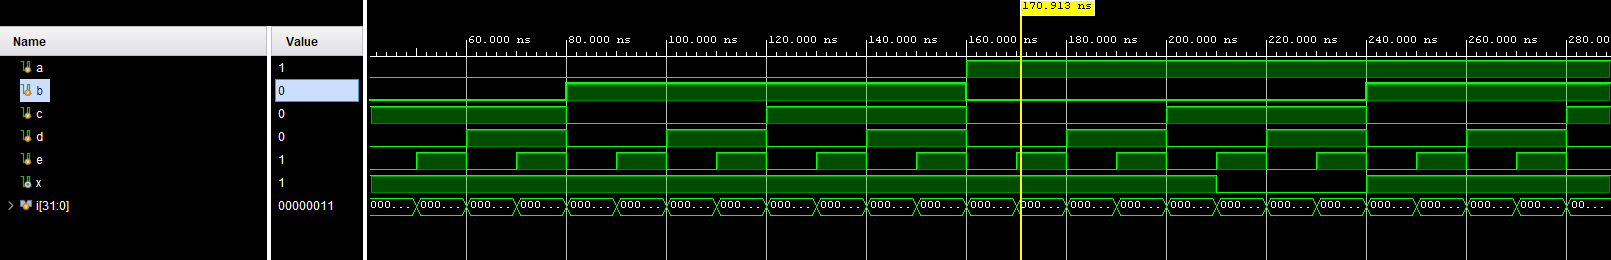
\includegraphics[width=1\textwidth]{multi_input_gate_waveform.png}
    \caption{多输入门电路仿真波形}
    \label{fig:tb_multi_input_gate}
\end{figure}

\begin{figure*}[p]
    \centering
    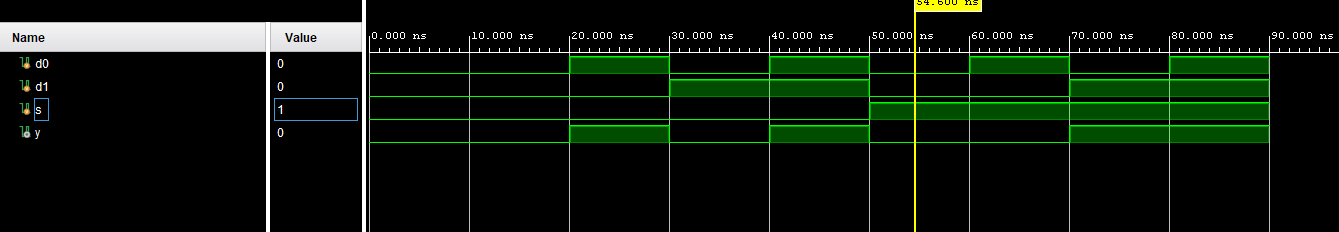
\includegraphics[width=1\textwidth]{two_way_mux_waveform.png}
    \caption{二路复用器仿真波形}
    \label{fig:tb_two_way_mux}
\end{figure}

\begin{figure*}[p]
    \centering
    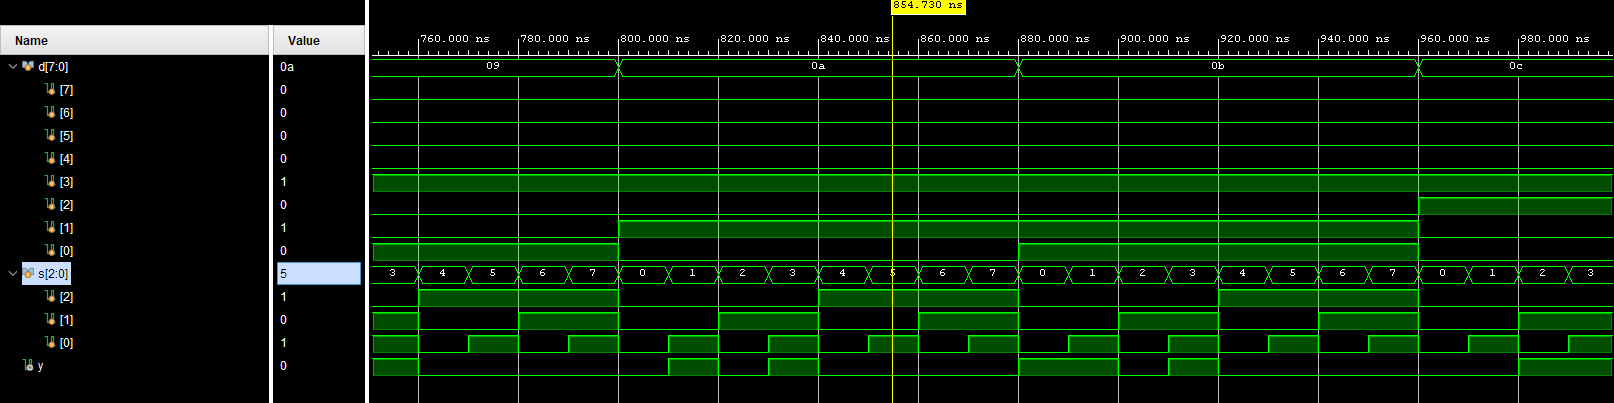
\includegraphics[width=1\textwidth]{eight_way_mux_waveform.png}
    \caption{八路复用器仿真波形}
    \label{fig:tb_eight_way_mux}
\end{figure}

\begin{figure*}[p]
    \centering
    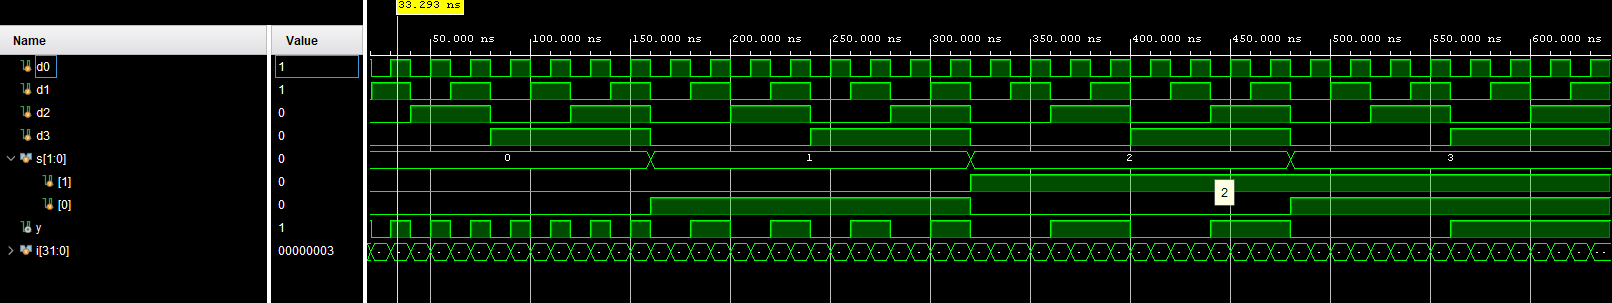
\includegraphics[width=1\textwidth]{four_way_mux_tristate_waveform.png}
    \caption{基于三态缓冲器的4路复用器仿真波形}
    \label{fig:tb_four_way_mux_tristate}
\end{figure}


\begin{figure*}[p]
    \centering
    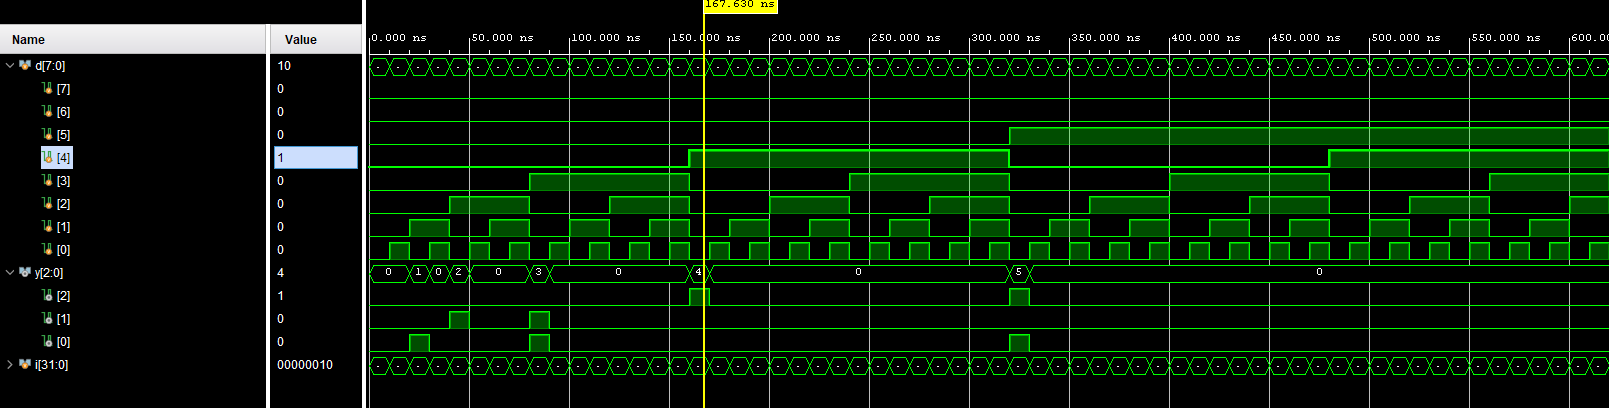
\includegraphics[width=1\textwidth]{encoder_8to3_waveform.png}
    \caption{8-3编码器仿真波形}
    \label{fig:tb_encoder_8to3}
\end{figure}

\clearpage 


\begin{figure*}[p]
    \centering
    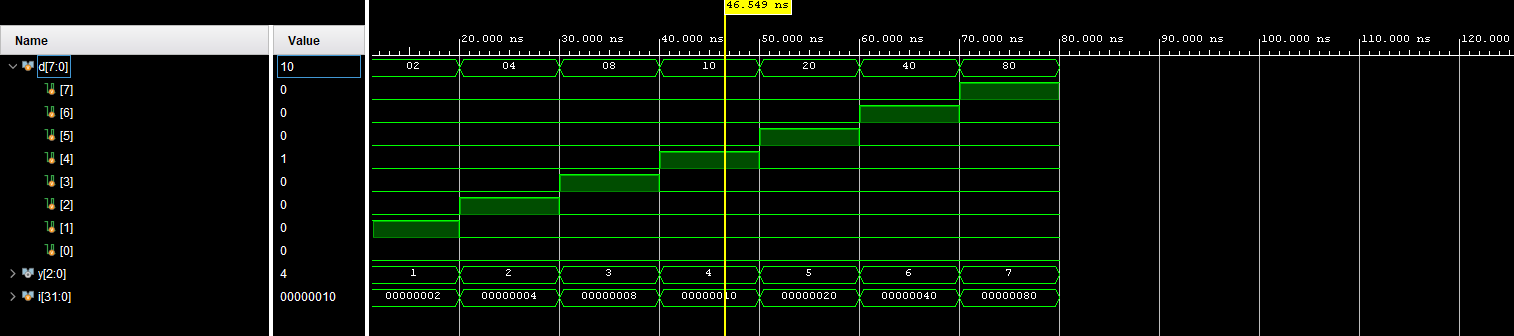
\includegraphics[width=1\textwidth]{encoder_8to3_ill_waveform.png}
    \caption{8-3编码器仿真波形}
    \label{fig:tb_encoder_8to3}
\end{figure}

\begin{figure*}[p]
    \centering
    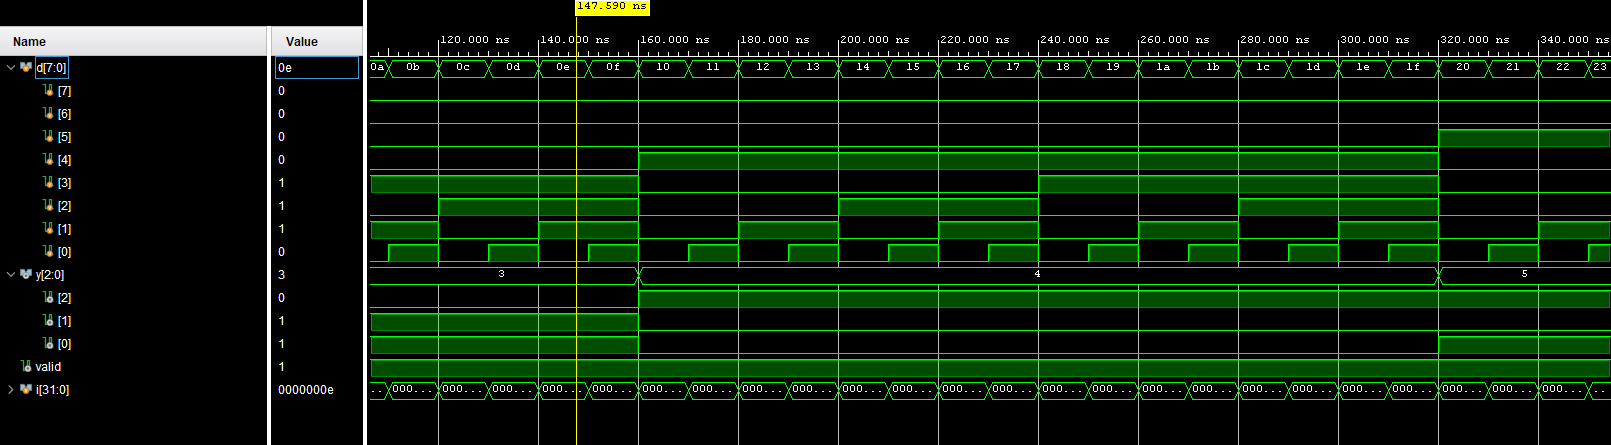
\includegraphics[width=1\textwidth]{priority_encoder_8to3_waveform.png}
    \caption{8-3优先编码器仿真波形}
    \label{fig:tb_priority_encoder_8to3}
\end{figure}

\begin{figure*}[p]
    \centering
    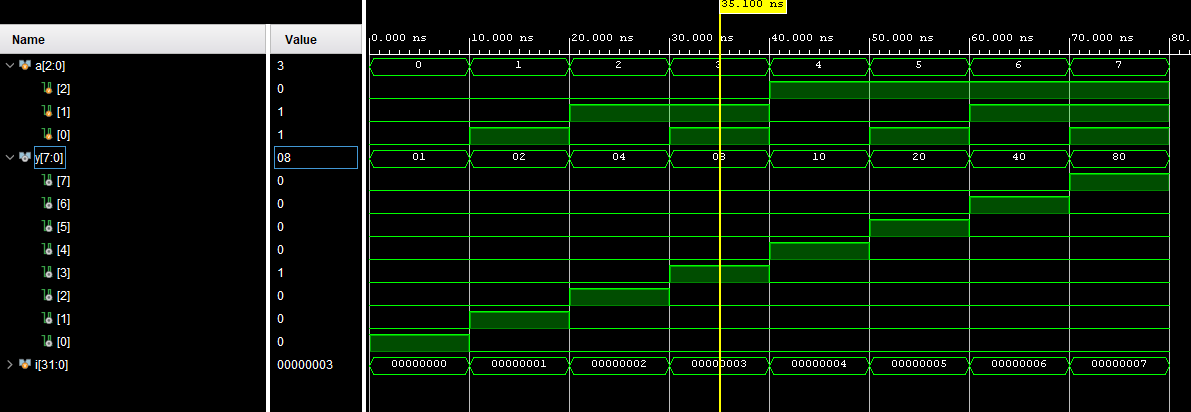
\includegraphics[width=1\textwidth]{decoder_3to8_waveform.png}
    \caption{3-8 译码器仿真波形}
    \label{fig:tb_decoder_3to8}
\end{figure}

%----------------------------------------------------------

\printbibliography

%----------------------------------------------------------



\end{document}